% Created by tikzDevice version 0.12.6 on 2025-01-17 13:26:52
% !TEX encoding = UTF-8 Unicode
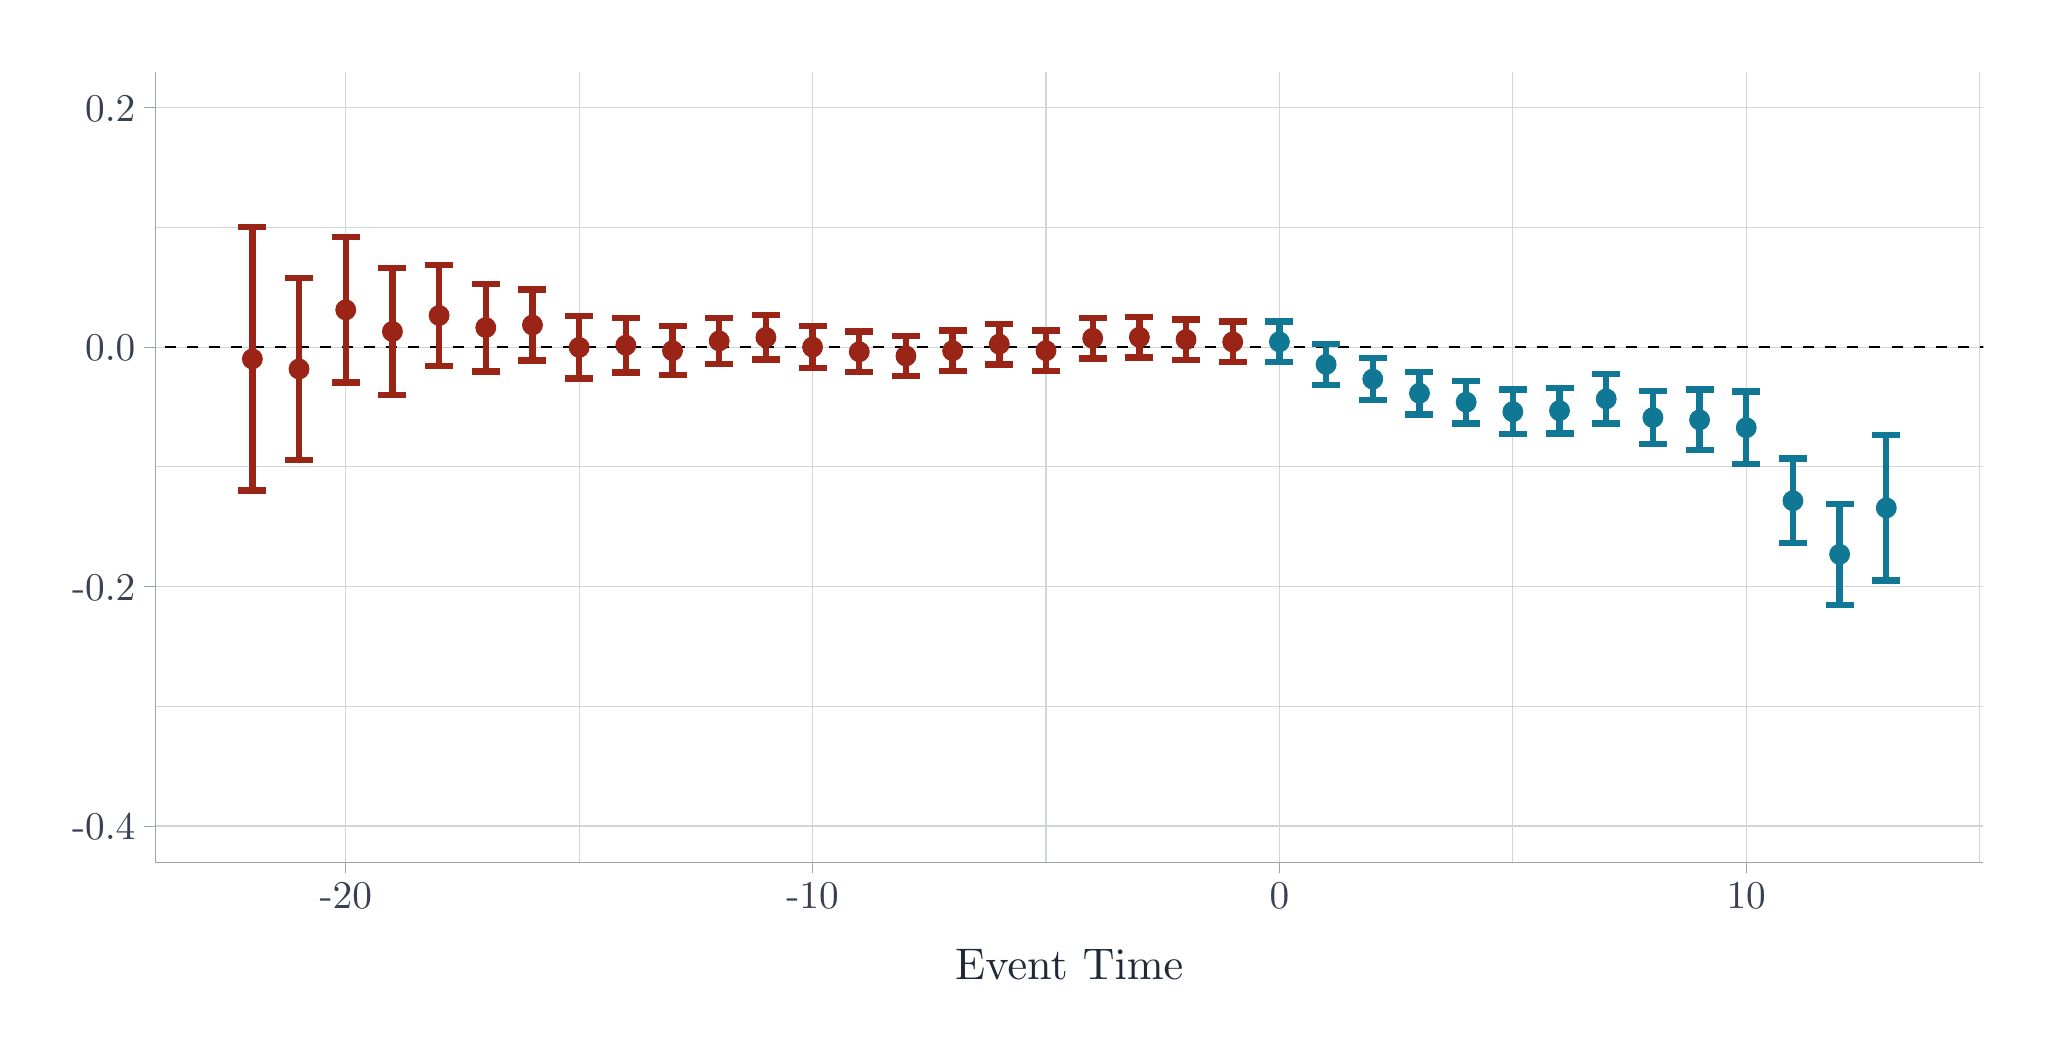
\begin{tikzpicture}[x=1pt,y=1pt]
\definecolor{fillColor}{RGB}{255,255,255}
\path[use as bounding box,fill=fillColor] (0,0) rectangle (722.70,361.35);
\begin{scope}
\path[clip] (  0.00,  0.00) rectangle (722.70,361.35);
\definecolor{drawColor}{RGB}{255,255,255}

\path[draw=drawColor,line width= 0.8pt,line join=round,line cap=round,fill=fillColor] (  0.00,  0.00) rectangle (722.70,361.35);
\end{scope}
\begin{scope}
\path[clip] ( 46.10, 59.89) rectangle (706.70,345.35);
\definecolor{drawColor}{RGB}{255,255,255}
\definecolor{fillColor}{RGB}{255,255,255}

\path[draw=drawColor,line width= 0.8pt,line join=round,line cap=round,fill=fillColor] ( 46.10, 59.89) rectangle (706.70,345.35);
\definecolor{drawColor}{RGB}{209,213,219}

\path[draw=drawColor,line width= 0.4pt,line join=round] ( 46.10,116.12) --
	(706.70,116.12);

\path[draw=drawColor,line width= 0.4pt,line join=round] ( 46.10,202.62) --
	(706.70,202.62);

\path[draw=drawColor,line width= 0.4pt,line join=round] ( 46.10,289.12) --
	(706.70,289.12);

\path[draw=drawColor,line width= 0.4pt,line join=round] (199.28, 59.89) --
	(199.28,345.35);

\path[draw=drawColor,line width= 0.4pt,line join=round] (367.97, 59.89) --
	(367.97,345.35);

\path[draw=drawColor,line width= 0.4pt,line join=round] (536.66, 59.89) --
	(536.66,345.35);

\path[draw=drawColor,line width= 0.4pt,line join=round] (705.35, 59.89) --
	(705.35,345.35);

\path[draw=drawColor,line width= 0.4pt,line join=round] ( 46.10, 72.86) --
	(706.70, 72.86);

\path[draw=drawColor,line width= 0.4pt,line join=round] ( 46.10,159.37) --
	(706.70,159.37);

\path[draw=drawColor,line width= 0.4pt,line join=round] ( 46.10,245.87) --
	(706.70,245.87);

\path[draw=drawColor,line width= 0.4pt,line join=round] ( 46.10,332.37) --
	(706.70,332.37);

\path[draw=drawColor,line width= 0.4pt,line join=round] (114.93, 59.89) --
	(114.93,345.35);

\path[draw=drawColor,line width= 0.4pt,line join=round] (283.62, 59.89) --
	(283.62,345.35);

\path[draw=drawColor,line width= 0.4pt,line join=round] (452.31, 59.89) --
	(452.31,345.35);

\path[draw=drawColor,line width= 0.4pt,line join=round] (621.00, 59.89) --
	(621.00,345.35);
\definecolor{drawColor}{RGB}{0,0,0}

\path[draw=drawColor,line width= 0.9pt,dash pattern=on 4pt off 4pt ,line join=round] (-614.49,245.87) -- (1367.30,245.87);
\definecolor{drawColor}{RGB}{154,36,21}
\definecolor{fillColor}{RGB}{154,36,21}

\path[draw=drawColor,line width= 0.4pt,line join=round,line cap=round,fill=fillColor] ( 81.19,241.65) circle (  3.57);

\path[draw=drawColor,line width= 0.4pt,line join=round,line cap=round,fill=fillColor] ( 98.06,238.01) circle (  3.57);

\path[draw=drawColor,line width= 0.4pt,line join=round,line cap=round,fill=fillColor] (114.93,259.37) circle (  3.57);

\path[draw=drawColor,line width= 0.4pt,line join=round,line cap=round,fill=fillColor] (131.80,251.55) circle (  3.57);

\path[draw=drawColor,line width= 0.4pt,line join=round,line cap=round,fill=fillColor] (148.67,257.36) circle (  3.57);

\path[draw=drawColor,line width= 0.4pt,line join=round,line cap=round,fill=fillColor] (165.54,252.97) circle (  3.57);

\path[draw=drawColor,line width= 0.4pt,line join=round,line cap=round,fill=fillColor] (182.41,253.91) circle (  3.57);

\path[draw=drawColor,line width= 0.4pt,line join=round,line cap=round,fill=fillColor] (199.28,245.82) circle (  3.57);

\path[draw=drawColor,line width= 0.4pt,line join=round,line cap=round,fill=fillColor] (216.15,246.60) circle (  3.57);

\path[draw=drawColor,line width= 0.4pt,line join=round,line cap=round,fill=fillColor] (233.01,244.61) circle (  3.57);

\path[draw=drawColor,line width= 0.4pt,line join=round,line cap=round,fill=fillColor] (249.88,248.15) circle (  3.57);

\path[draw=drawColor,line width= 0.4pt,line join=round,line cap=round,fill=fillColor] (266.75,249.43) circle (  3.57);

\path[draw=drawColor,line width= 0.4pt,line join=round,line cap=round,fill=fillColor] (283.62,245.92) circle (  3.57);

\path[draw=drawColor,line width= 0.4pt,line join=round,line cap=round,fill=fillColor] (300.49,244.24) circle (  3.57);

\path[draw=drawColor,line width= 0.4pt,line join=round,line cap=round,fill=fillColor] (317.36,242.71) circle (  3.57);

\path[draw=drawColor,line width= 0.4pt,line join=round,line cap=round,fill=fillColor] (334.23,244.59) circle (  3.57);

\path[draw=drawColor,line width= 0.4pt,line join=round,line cap=round,fill=fillColor] (351.10,247.01) circle (  3.57);

\path[draw=drawColor,line width= 0.4pt,line join=round,line cap=round,fill=fillColor] (367.97,244.63) circle (  3.57);

\path[draw=drawColor,line width= 0.4pt,line join=round,line cap=round,fill=fillColor] (384.84,249.11) circle (  3.57);

\path[draw=drawColor,line width= 0.4pt,line join=round,line cap=round,fill=fillColor] (401.71,249.49) circle (  3.57);

\path[draw=drawColor,line width= 0.4pt,line join=round,line cap=round,fill=fillColor] (418.58,248.64) circle (  3.57);

\path[draw=drawColor,line width= 0.4pt,line join=round,line cap=round,fill=fillColor] (435.44,247.79) circle (  3.57);
\definecolor{drawColor}{RGB}{16,120,149}
\definecolor{fillColor}{RGB}{16,120,149}

\path[draw=drawColor,line width= 0.4pt,line join=round,line cap=round,fill=fillColor] (452.31,247.82) circle (  3.57);

\path[draw=drawColor,line width= 0.4pt,line join=round,line cap=round,fill=fillColor] (469.18,239.68) circle (  3.57);

\path[draw=drawColor,line width= 0.4pt,line join=round,line cap=round,fill=fillColor] (486.05,234.37) circle (  3.57);

\path[draw=drawColor,line width= 0.4pt,line join=round,line cap=round,fill=fillColor] (502.92,229.26) circle (  3.57);

\path[draw=drawColor,line width= 0.4pt,line join=round,line cap=round,fill=fillColor] (519.79,226.02) circle (  3.57);

\path[draw=drawColor,line width= 0.4pt,line join=round,line cap=round,fill=fillColor] (536.66,222.56) circle (  3.57);

\path[draw=drawColor,line width= 0.4pt,line join=round,line cap=round,fill=fillColor] (553.53,222.94) circle (  3.57);

\path[draw=drawColor,line width= 0.4pt,line join=round,line cap=round,fill=fillColor] (570.40,227.20) circle (  3.57);

\path[draw=drawColor,line width= 0.4pt,line join=round,line cap=round,fill=fillColor] (587.27,220.46) circle (  3.57);

\path[draw=drawColor,line width= 0.4pt,line join=round,line cap=round,fill=fillColor] (604.14,219.62) circle (  3.57);

\path[draw=drawColor,line width= 0.4pt,line join=round,line cap=round,fill=fillColor] (621.00,216.79) circle (  3.57);

\path[draw=drawColor,line width= 0.4pt,line join=round,line cap=round,fill=fillColor] (637.87,190.39) circle (  3.57);

\path[draw=drawColor,line width= 0.4pt,line join=round,line cap=round,fill=fillColor] (654.74,171.06) circle (  3.57);

\path[draw=drawColor,line width= 0.4pt,line join=round,line cap=round,fill=fillColor] (671.61,187.81) circle (  3.57);
\definecolor{drawColor}{RGB}{154,36,21}

\path[draw=drawColor,line width= 2.3pt,line join=round] ( 76.13,289.24) --
	( 86.25,289.24);

\path[draw=drawColor,line width= 2.3pt,line join=round] ( 81.19,289.24) --
	( 81.19,194.07);

\path[draw=drawColor,line width= 2.3pt,line join=round] ( 76.13,194.07) --
	( 86.25,194.07);

\path[draw=drawColor,line width= 2.3pt,line join=round] ( 93.00,270.88) --
	(103.12,270.88);

\path[draw=drawColor,line width= 2.3pt,line join=round] ( 98.06,270.88) --
	( 98.06,205.14);

\path[draw=drawColor,line width= 2.3pt,line join=round] ( 93.00,205.14) --
	(103.12,205.14);

\path[draw=drawColor,line width= 2.3pt,line join=round] (109.87,285.62) --
	(119.99,285.62);

\path[draw=drawColor,line width= 2.3pt,line join=round] (114.93,285.62) --
	(114.93,233.12);

\path[draw=drawColor,line width= 2.3pt,line join=round] (109.87,233.12) --
	(119.99,233.12);

\path[draw=drawColor,line width= 2.3pt,line join=round] (126.74,274.41) --
	(136.86,274.41);

\path[draw=drawColor,line width= 2.3pt,line join=round] (131.80,274.41) --
	(131.80,228.70);

\path[draw=drawColor,line width= 2.3pt,line join=round] (126.74,228.70) --
	(136.86,228.70);

\path[draw=drawColor,line width= 2.3pt,line join=round] (143.61,275.54) --
	(153.73,275.54);

\path[draw=drawColor,line width= 2.3pt,line join=round] (148.67,275.54) --
	(148.67,239.19);

\path[draw=drawColor,line width= 2.3pt,line join=round] (143.61,239.19) --
	(153.73,239.19);

\path[draw=drawColor,line width= 2.3pt,line join=round] (160.48,268.79) --
	(170.60,268.79);

\path[draw=drawColor,line width= 2.3pt,line join=round] (165.54,268.79) --
	(165.54,237.15);

\path[draw=drawColor,line width= 2.3pt,line join=round] (160.48,237.15) --
	(170.60,237.15);

\path[draw=drawColor,line width= 2.3pt,line join=round] (177.35,266.78) --
	(187.47,266.78);

\path[draw=drawColor,line width= 2.3pt,line join=round] (182.41,266.78) --
	(182.41,241.04);

\path[draw=drawColor,line width= 2.3pt,line join=round] (177.35,241.04) --
	(187.47,241.04);

\path[draw=drawColor,line width= 2.3pt,line join=round] (194.22,257.08) --
	(204.34,257.08);

\path[draw=drawColor,line width= 2.3pt,line join=round] (199.28,257.08) --
	(199.28,234.56);

\path[draw=drawColor,line width= 2.3pt,line join=round] (194.22,234.56) --
	(204.34,234.56);

\path[draw=drawColor,line width= 2.3pt,line join=round] (211.08,256.47) --
	(221.21,256.47);

\path[draw=drawColor,line width= 2.3pt,line join=round] (216.15,256.47) --
	(216.15,236.73);

\path[draw=drawColor,line width= 2.3pt,line join=round] (211.08,236.73) --
	(221.21,236.73);

\path[draw=drawColor,line width= 2.3pt,line join=round] (227.95,253.47) --
	(238.08,253.47);

\path[draw=drawColor,line width= 2.3pt,line join=round] (233.01,253.47) --
	(233.01,235.75);

\path[draw=drawColor,line width= 2.3pt,line join=round] (227.95,235.75) --
	(238.08,235.75);

\path[draw=drawColor,line width= 2.3pt,line join=round] (244.82,256.49) --
	(254.94,256.49);

\path[draw=drawColor,line width= 2.3pt,line join=round] (249.88,256.49) --
	(249.88,239.80);

\path[draw=drawColor,line width= 2.3pt,line join=round] (244.82,239.80) --
	(254.94,239.80);

\path[draw=drawColor,line width= 2.3pt,line join=round] (261.69,257.42) --
	(271.81,257.42);

\path[draw=drawColor,line width= 2.3pt,line join=round] (266.75,257.42) --
	(266.75,241.43);

\path[draw=drawColor,line width= 2.3pt,line join=round] (261.69,241.43) --
	(271.81,241.43);

\path[draw=drawColor,line width= 2.3pt,line join=round] (278.56,253.55) --
	(288.68,253.55);

\path[draw=drawColor,line width= 2.3pt,line join=round] (283.62,253.55) --
	(283.62,238.29);

\path[draw=drawColor,line width= 2.3pt,line join=round] (278.56,238.29) --
	(288.68,238.29);

\path[draw=drawColor,line width= 2.3pt,line join=round] (295.43,251.56) --
	(305.55,251.56);

\path[draw=drawColor,line width= 2.3pt,line join=round] (300.49,251.56) --
	(300.49,236.91);

\path[draw=drawColor,line width= 2.3pt,line join=round] (295.43,236.91) --
	(305.55,236.91);

\path[draw=drawColor,line width= 2.3pt,line join=round] (312.30,250.03) --
	(322.42,250.03);

\path[draw=drawColor,line width= 2.3pt,line join=round] (317.36,250.03) --
	(317.36,235.38);

\path[draw=drawColor,line width= 2.3pt,line join=round] (312.30,235.38) --
	(322.42,235.38);

\path[draw=drawColor,line width= 2.3pt,line join=round] (329.17,251.92) --
	(339.29,251.92);

\path[draw=drawColor,line width= 2.3pt,line join=round] (334.23,251.92) --
	(334.23,237.26);

\path[draw=drawColor,line width= 2.3pt,line join=round] (329.17,237.26) --
	(339.29,237.26);

\path[draw=drawColor,line width= 2.3pt,line join=round] (346.04,254.33) --
	(356.16,254.33);

\path[draw=drawColor,line width= 2.3pt,line join=round] (351.10,254.33) --
	(351.10,239.68);

\path[draw=drawColor,line width= 2.3pt,line join=round] (346.04,239.68) --
	(356.16,239.68);

\path[draw=drawColor,line width= 2.3pt,line join=round] (362.91,251.95) --
	(373.03,251.95);

\path[draw=drawColor,line width= 2.3pt,line join=round] (367.97,251.95) --
	(367.97,237.30);

\path[draw=drawColor,line width= 2.3pt,line join=round] (362.91,237.30) --
	(373.03,237.30);

\path[draw=drawColor,line width= 2.3pt,line join=round] (379.78,256.43) --
	(389.90,256.43);

\path[draw=drawColor,line width= 2.3pt,line join=round] (384.84,256.43) --
	(384.84,241.78);

\path[draw=drawColor,line width= 2.3pt,line join=round] (379.78,241.78) --
	(389.90,241.78);

\path[draw=drawColor,line width= 2.3pt,line join=round] (396.65,256.81) --
	(406.77,256.81);

\path[draw=drawColor,line width= 2.3pt,line join=round] (401.71,256.81) --
	(401.71,242.16);

\path[draw=drawColor,line width= 2.3pt,line join=round] (396.65,242.16) --
	(406.77,242.16);

\path[draw=drawColor,line width= 2.3pt,line join=round] (413.51,255.96) --
	(423.64,255.96);

\path[draw=drawColor,line width= 2.3pt,line join=round] (418.58,255.96) --
	(418.58,241.31);

\path[draw=drawColor,line width= 2.3pt,line join=round] (413.51,241.31) --
	(423.64,241.31);

\path[draw=drawColor,line width= 2.3pt,line join=round] (430.38,255.11) --
	(440.50,255.11);

\path[draw=drawColor,line width= 2.3pt,line join=round] (435.44,255.11) --
	(435.44,240.46);

\path[draw=drawColor,line width= 2.3pt,line join=round] (430.38,240.46) --
	(440.50,240.46);
\definecolor{drawColor}{RGB}{16,120,149}

\path[draw=drawColor,line width= 2.3pt,line join=round] (447.25,255.15) --
	(457.37,255.15);

\path[draw=drawColor,line width= 2.3pt,line join=round] (452.31,255.15) --
	(452.31,240.50);

\path[draw=drawColor,line width= 2.3pt,line join=round] (447.25,240.50) --
	(457.37,240.50);

\path[draw=drawColor,line width= 2.3pt,line join=round] (464.12,247.09) --
	(474.24,247.09);

\path[draw=drawColor,line width= 2.3pt,line join=round] (469.18,247.09) --
	(469.18,232.27);

\path[draw=drawColor,line width= 2.3pt,line join=round] (464.12,232.27) --
	(474.24,232.27);

\path[draw=drawColor,line width= 2.3pt,line join=round] (480.99,241.88) --
	(491.11,241.88);

\path[draw=drawColor,line width= 2.3pt,line join=round] (486.05,241.88) --
	(486.05,226.86);

\path[draw=drawColor,line width= 2.3pt,line join=round] (480.99,226.86) --
	(491.11,226.86);

\path[draw=drawColor,line width= 2.3pt,line join=round] (497.86,236.89) --
	(507.98,236.89);

\path[draw=drawColor,line width= 2.3pt,line join=round] (502.92,236.89) --
	(502.92,221.63);

\path[draw=drawColor,line width= 2.3pt,line join=round] (497.86,221.63) --
	(507.98,221.63);

\path[draw=drawColor,line width= 2.3pt,line join=round] (514.73,233.75) --
	(524.85,233.75);

\path[draw=drawColor,line width= 2.3pt,line join=round] (519.79,233.75) --
	(519.79,218.28);

\path[draw=drawColor,line width= 2.3pt,line join=round] (514.73,218.28) --
	(524.85,218.28);

\path[draw=drawColor,line width= 2.3pt,line join=round] (531.60,230.56) --
	(541.72,230.56);

\path[draw=drawColor,line width= 2.3pt,line join=round] (536.66,230.56) --
	(536.66,214.56);

\path[draw=drawColor,line width= 2.3pt,line join=round] (531.60,214.56) --
	(541.72,214.56);

\path[draw=drawColor,line width= 2.3pt,line join=round] (548.47,231.20) --
	(558.59,231.20);

\path[draw=drawColor,line width= 2.3pt,line join=round] (553.53,231.20) --
	(553.53,214.67);

\path[draw=drawColor,line width= 2.3pt,line join=round] (548.47,214.67) --
	(558.59,214.67);

\path[draw=drawColor,line width= 2.3pt,line join=round] (565.34,236.11) --
	(575.46,236.11);

\path[draw=drawColor,line width= 2.3pt,line join=round] (570.40,236.11) --
	(570.40,218.29);

\path[draw=drawColor,line width= 2.3pt,line join=round] (565.34,218.29) --
	(575.46,218.29);

\path[draw=drawColor,line width= 2.3pt,line join=round] (582.21,230.10) --
	(592.33,230.10);

\path[draw=drawColor,line width= 2.3pt,line join=round] (587.27,230.10) --
	(587.27,210.81);

\path[draw=drawColor,line width= 2.3pt,line join=round] (582.21,210.81) --
	(592.33,210.81);

\path[draw=drawColor,line width= 2.3pt,line join=round] (599.07,230.55) --
	(609.20,230.55);

\path[draw=drawColor,line width= 2.3pt,line join=round] (604.14,230.55) --
	(604.14,208.69);

\path[draw=drawColor,line width= 2.3pt,line join=round] (599.07,208.69) --
	(609.20,208.69);

\path[draw=drawColor,line width= 2.3pt,line join=round] (615.94,229.82) --
	(626.07,229.82);

\path[draw=drawColor,line width= 2.3pt,line join=round] (621.00,229.82) --
	(621.00,203.76);

\path[draw=drawColor,line width= 2.3pt,line join=round] (615.94,203.76) --
	(626.07,203.76);

\path[draw=drawColor,line width= 2.3pt,line join=round] (632.81,205.69) --
	(642.93,205.69);

\path[draw=drawColor,line width= 2.3pt,line join=round] (637.87,205.69) --
	(637.87,175.08);

\path[draw=drawColor,line width= 2.3pt,line join=round] (632.81,175.08) --
	(642.93,175.08);

\path[draw=drawColor,line width= 2.3pt,line join=round] (649.68,189.30) --
	(659.80,189.30);

\path[draw=drawColor,line width= 2.3pt,line join=round] (654.74,189.30) --
	(654.74,152.83);

\path[draw=drawColor,line width= 2.3pt,line join=round] (649.68,152.83) --
	(659.80,152.83);

\path[draw=drawColor,line width= 2.3pt,line join=round] (666.55,214.06) --
	(676.67,214.06);

\path[draw=drawColor,line width= 2.3pt,line join=round] (671.61,214.06) --
	(671.61,161.57);

\path[draw=drawColor,line width= 2.3pt,line join=round] (666.55,161.57) --
	(676.67,161.57);
\end{scope}
\begin{scope}
\path[clip] (  0.00,  0.00) rectangle (722.70,361.35);
\definecolor{drawColor}{RGB}{156,163,175}

\path[draw=drawColor,line width= 0.3pt,line join=round] ( 46.10, 59.89) --
	( 46.10,345.35);
\end{scope}
\begin{scope}
\path[clip] (  0.00,  0.00) rectangle (722.70,361.35);
\definecolor{drawColor}{RGB}{55,65,81}

\node[text=drawColor,anchor=base east,inner sep=0pt, outer sep=0pt, scale=  1.42] at ( 38.90, 67.97) {-0.4};

\node[text=drawColor,anchor=base east,inner sep=0pt, outer sep=0pt, scale=  1.42] at ( 38.90,154.47) {-0.2};

\node[text=drawColor,anchor=base east,inner sep=0pt, outer sep=0pt, scale=  1.42] at ( 38.90,240.97) {0.0};

\node[text=drawColor,anchor=base east,inner sep=0pt, outer sep=0pt, scale=  1.42] at ( 38.90,327.48) {0.2};
\end{scope}
\begin{scope}
\path[clip] (  0.00,  0.00) rectangle (722.70,361.35);
\definecolor{drawColor}{RGB}{156,163,175}

\path[draw=drawColor,line width= 0.3pt,line join=round] ( 42.10, 72.86) --
	( 46.10, 72.86);

\path[draw=drawColor,line width= 0.3pt,line join=round] ( 42.10,159.37) --
	( 46.10,159.37);

\path[draw=drawColor,line width= 0.3pt,line join=round] ( 42.10,245.87) --
	( 46.10,245.87);

\path[draw=drawColor,line width= 0.3pt,line join=round] ( 42.10,332.37) --
	( 46.10,332.37);
\end{scope}
\begin{scope}
\path[clip] (  0.00,  0.00) rectangle (722.70,361.35);
\definecolor{drawColor}{RGB}{156,163,175}

\path[draw=drawColor,line width= 0.3pt,line join=round] ( 46.10, 59.89) --
	(706.70, 59.89);
\end{scope}
\begin{scope}
\path[clip] (  0.00,  0.00) rectangle (722.70,361.35);
\definecolor{drawColor}{RGB}{156,163,175}

\path[draw=drawColor,line width= 0.3pt,line join=round] (114.93, 55.89) --
	(114.93, 59.89);

\path[draw=drawColor,line width= 0.3pt,line join=round] (283.62, 55.89) --
	(283.62, 59.89);

\path[draw=drawColor,line width= 0.3pt,line join=round] (452.31, 55.89) --
	(452.31, 59.89);

\path[draw=drawColor,line width= 0.3pt,line join=round] (621.00, 55.89) --
	(621.00, 59.89);
\end{scope}
\begin{scope}
\path[clip] (  0.00,  0.00) rectangle (722.70,361.35);
\definecolor{drawColor}{RGB}{55,65,81}

\node[text=drawColor,anchor=base,inner sep=0pt, outer sep=0pt, scale=  1.42] at (114.93, 42.89) {-20};

\node[text=drawColor,anchor=base,inner sep=0pt, outer sep=0pt, scale=  1.42] at (283.62, 42.89) {-10};

\node[text=drawColor,anchor=base,inner sep=0pt, outer sep=0pt, scale=  1.42] at (452.31, 42.89) {0};

\node[text=drawColor,anchor=base,inner sep=0pt, outer sep=0pt, scale=  1.42] at (621.00, 42.89) {10};
\end{scope}
\begin{scope}
\path[clip] (  0.00,  0.00) rectangle (722.70,361.35);
\definecolor{drawColor}{RGB}{31,41,55}

\node[text=drawColor,anchor=base,inner sep=0pt, outer sep=0pt, scale=  1.60] at (376.40, 17.56) {Event Time};
\end{scope}
\end{tikzpicture}
